%% This is the ctufit-thesis example file. It is used to produce theses
%% for submission to Czech Technical University, Faculty of Information Technology.
%%
%% This is version 1.3.8, built 29. 10. 2024.
%% 
%% Get the newest version from
%% https://gitlab.fit.cvut.cz/theses-templates/FITthesis-LaTeX
%%
%%
%% Copyright 2024, Tomas Novacek
%% Copyright 2021, Eliska Sestakova and Ondrej Guth
%%
%% This work may be distributed and/or modified under the
%% conditions of the LaTeX Project Public License, either version 1.3
%% of this license or (at your option) any later version.
%% The latest version of this license is in
%%  https://www.latex-project.org/lppl.txt
%% and version 1.3 or later is part of all distributions of LaTeX
%% version 2005/12/01 or later.
%%
%% This work has the LPPL maintenance status `maintained'.
%%
%% The current maintainer of this work is Tomas Novacek.
%% Alternatively, submit bug reports to the tracker at
%% https://gitlab.fit.cvut.cz/theses-templates/FITthesis-LaTeX/issues
%%
%%

% arara: xelatex
% arara: biber
% arara: xelatex
% arara: xelatex

%%%%%%%%%%%%%%%%%%%%%%%%%%%%%%%%%%%%%%%%%
% CLASS OPTIONS
% language: czech/english/slovak
% thesis type: bachelor/master/dissertation
% colour: bw for black&white OR no option for default colour scheme
% electronic (oneside) or printed (twoside), twoside is default
% paragraph - if passed, this optional argument sets paragraphs as the deepest level of headers, styles it, numbers it and adds it to Table of Content. Use with care! Normally, it is considered unwise to use it, since its too deep.
%%%%%%%%%%%%%%%%%%%%%%%%%%%%%%%%%%%%%%%%%
\documentclass[czech,master,unicode,oneside]{ctufit-thesis}

%%%%%%%%%%%%%%%%%%%%%%%%%%%%%%%%%%
% FILL IN THIS INFORMATION
%%%%%%%%%%%%%%%%%%%%%%%%%%%%%%%%%%
\ctufittitle{Webový gamifikační dashboard pro porovnání výkonnosti vývojářů} % replace with the title of your thesis
\ctufitauthorfull{Bc. Lukáš Paukert} % replace with your full name (first name(s) and then family name(s) / surname(s)) including academic degrees
\ctufitauthorsurnames{Paukert} % replace with your surname(s) / family name(s)
\ctufitauthorgivennames{Lukáš} % replace with your first name(s) / given name(s)
\ctufitsupervisor{Ing. Pavel Švagr} % replace with name of your supervisor/advisor (include academic degrees)
\ctufitdepartment{Katedra softwarového inženýrství} % replace with the department of your defence
\ctufityear{2026} % replace with the year of your defence
\ctufitdeclarationplace{Praze} % replace with the place where you sign the declaration
\ctufitdeclarationdate{\today} % replace with the date of signature of the declaration
\ctufitabstractCZE{Tato diplomová práce se zabývá návrhem a implementací open source webové aplikace sloužící k přehledné prezentaci aktivit vývojářů. Hlavním cílem práce je vytvoření nástroje pro efektivní monitorování metrik z procesu vývoje softwaru a následné porovnávání výkonnosti mezi vývojáři a vývojovými týmy.

V teoretické části je provedena rešerše existujících řešení a analýza metrik vhodných pro měření kvality a efektivity práce vývojářů. Pozornost je věnována výběru vhodných ukazatelů, které lze automatizovaně získávat z verzovacích systémů GitHub a GitLab prostřednictvím jejich API. Na základě získaných poznatků je navržen systém zajišťující konsolidaci dat z více zdrojů a jejich následné párování na konkrétní uživatelské účty.

Praktická část práce zahrnuje implementaci navrženého řešení ve frame\-worku Laravel s využitím knihovny Inertia.js a frontendového frameworku Vue.js. Výsledná aplikace poskytuje rozhraní pro správu uživatelů a vizualizaci dat ve formě přehledných grafů a tabulek. Součástí systému je rovněž modul pro definici výzev využívající principy gamifikace. Funkčnost výsledné aplikace byla ověřena v rámci uživatelského testování.}
\ctufitabstractENG{This master's thesis focuses on the design and implementation of an open source web application dedicated to the transparent presentation of developer activities. The primary objective of the work is to develop a tool for the efficient monitoring of software development process metrics and the subsequent performance comparison between individual developers and development teams.

The theoretical section provides a review of existing solutions and an analysis of metrics suitable for measuring the quality and efficiency of developers' work. Emphasis is placed on the selection of appropriate indicators that can be automatically retrieved from the GitHub and GitLab version control systems via their respective API. Based on the findings, a system is designed to ensure data consolidation from multiple sources and its subsequent mapping to specific user accounts.

The practical part of the thesis involves the implementation of the proposed solution using the Laravel framework, integrated with the Inertia.js library and the Vue.js frontend framework. The resulting application provides an interface for user management and data visualization in the form of intuitive charts and tables. Furthermore, the system includes a module for challenge definitions based on gamification principles. The functionality of the final application was verified through user testing.}
\ctufitkeywordsCZE{měření výkonnosti vývojářů, metriky, gamifikace, single-page webová aplikace, GitHub, GitLab, Laravel, Vue.js, Inertia.js}
\ctufitkeywordsENG{measuring developer performance, metrics, gamification, single-page web application, GitHub, GitLab, Laravel, Vue.js, Inertia.js}
%%%%%%%%%%%%%%%%%%%%%%%%%%%%%%%%%%
% END FILL IN
%%%%%%%%%%%%%%%%%%%%%%%%%%%%%%%%%%

%%%%%%%%%%%%%%%%%%%%%%%%%%%%%%%%%%
% CUSTOMIZATION of this template
% Skip this part or alter it if you know what you are doing.
%%%%%%%%%%%%%%%%%%%%%%%%%%%%%%%%%%

\RequirePackage{iftex}[2020/03/06]
\iftutex % XeLaTeX and LuaLaTeX
    \RequirePackage{ellipsis}[2020/05/22] %ellipsis workaround for XeLaTeX
\else
    \errmessage{Only compilation with XeLaTeX or LuaLaTeX is allowed}
    \stop
\fi

% hyperlinks
\hypersetup{
    pdfpagelayout=TwoPageRight,
    colorlinks=false,
    allcolors=decoration,
    pdfborder={0 0 0.1}
}

% uncomment the following to hide all hyperlinks
%\hypersetup{hidelinks}

% uncomment the following to change the colour of all hyperlinks to CTU blue
%\hypersetup{allbordercolors=decoration}

\RequirePackage{pdfpages}[2020/01/28]

%%%%%%%%%%%%%%%%%%%%%%%%%%%%%%%%%%
% CUSTOMIZATION of this template END
%%%%%%%%%%%%%%%%%%%%%%%%%%%%%%%%%%


%%%%%%%%%%%%%%%%%%%%%%
% DEMO CONTENTS SETTINGS
% You may choose to modify this part.
%%%%%%%%%%%%%%%%%%%%%%
\usepackage{dirtree}
\usepackage{lipsum,tikz}
\usepackage[style=iso-numeric]{biblatex}
\addbibresource{other/bib-database.bib}
\usepackage{xurl}
%\usepackage{listings} % typesetting of sources
\usepackage{minted}
\captionsetup[listing]{position=top, skip=1pt}
\usepackage{csquotes}
\usepackage[textsize=tiny]{todonotes}
\usepackage{xevlna}
\usepackage{pdflscape}
\usepackage[export]{adjustbox}
\definecolor{gray}{HTML}{DCDCDC}

% word wrap
\hyphenation{GitHub}
\hyphenation{GitLab}
\hyphenation{commit commitů}
\hyphenation{DevOps}
\hyphenation{Duolingo}
\hyphenation{JavaScript JavaScriptové JavaScriptová JavaScriptovou}
\hyphenation{GraphQL}

% macros
\usepackage{enumitem}
\newcommand{\myItem}[1]{\item{\textbf{#1}}\\[1mm]}

\usepackage{tabularx}
\newcolumntype{L}{>{\raggedright\arraybackslash}X}
\newcolumntype{R}{>{\raggedleft\arraybackslash}X}
\newcolumntype{C}{>{\centering\arraybackslash}X}

%%%%%%%%%%%%%%%%%%%%%%
% DEMO CONTENTS SETTINGS END
%%%%%%%%%%%%%%%%%%%%%%

\begin{document} 
\frontmatter\frontmatterinit % do not remove these two commands

\thispagestyle{empty}\maketitle\thispagestyle{empty}\cleardoublepage % do not remove these four commands

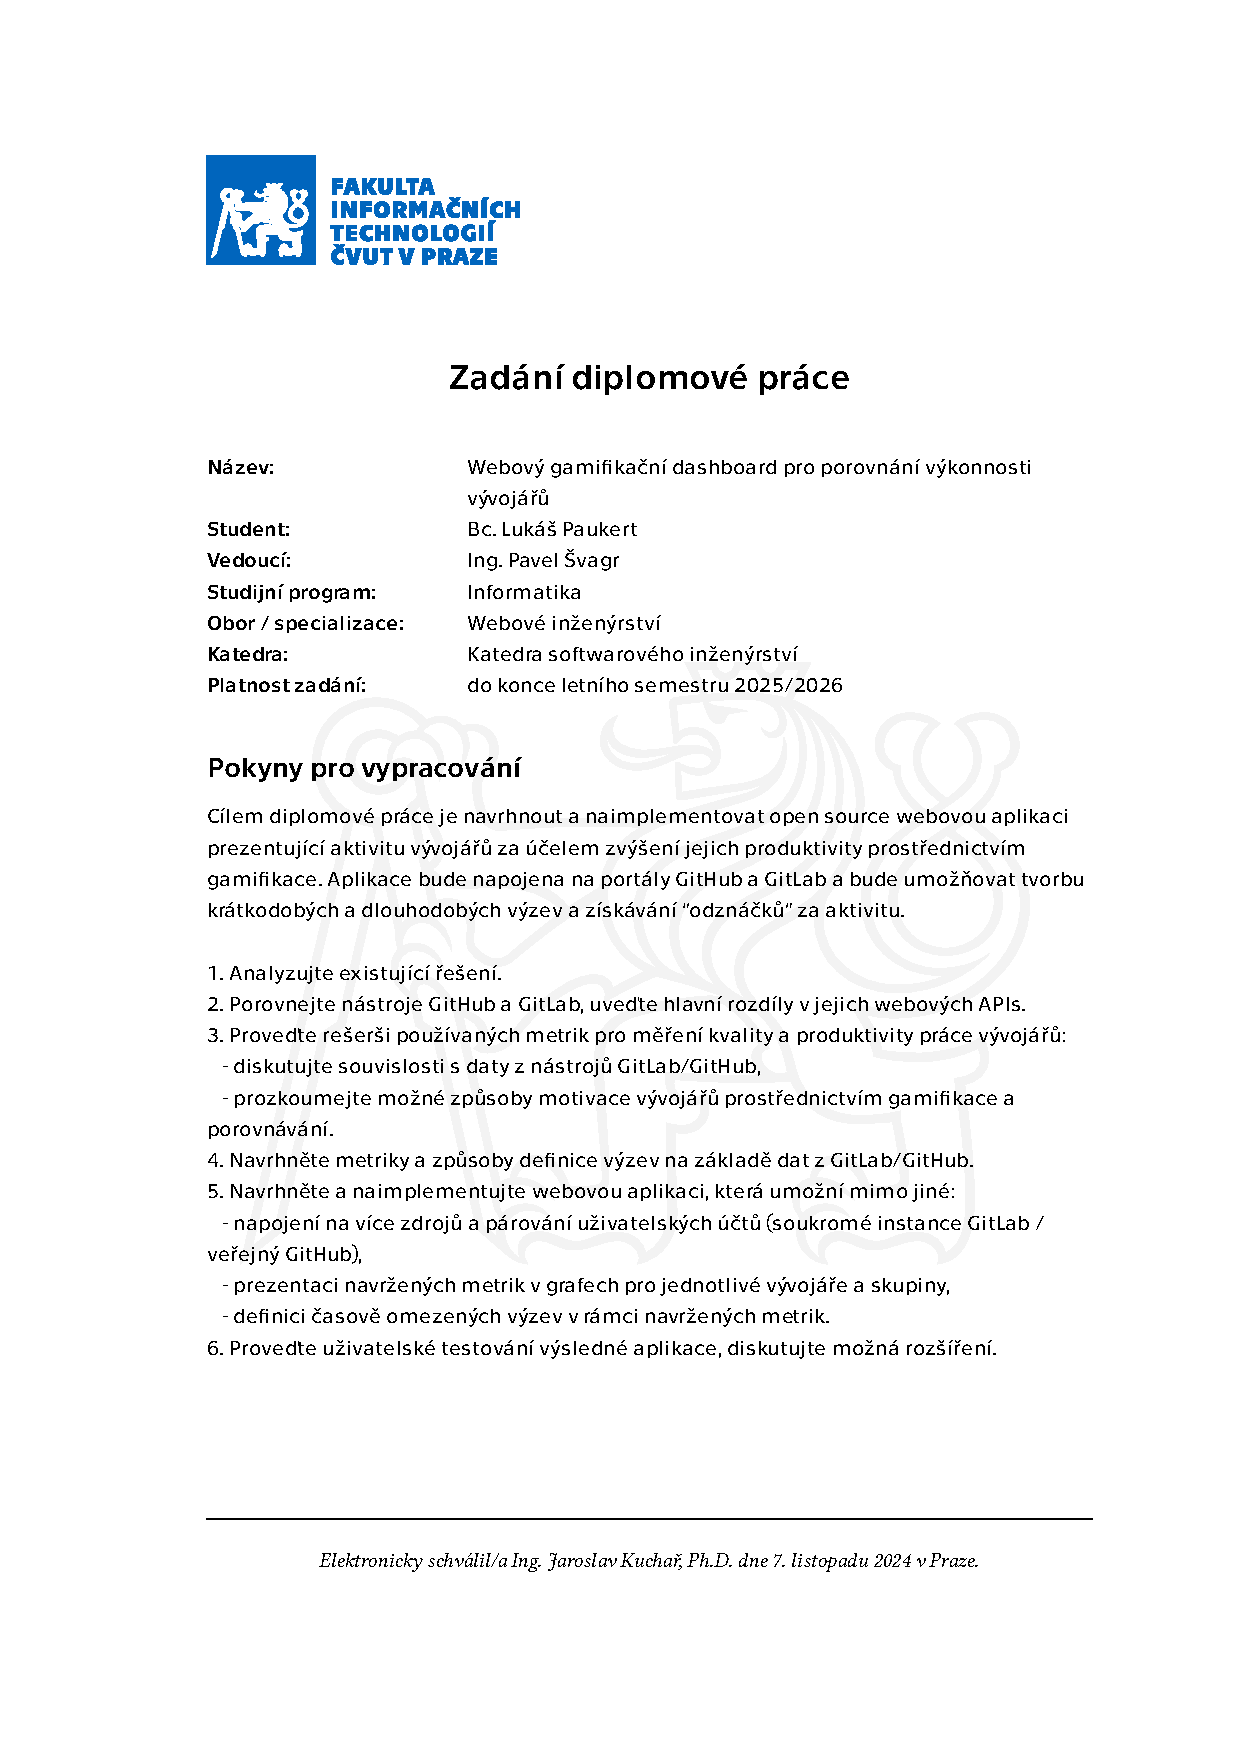
\includepdf[pages={1-}]{assignment-include.pdf} % replace this file with your thesis assignment generated from ProjectsFIT

\imprintpage % do not remove this command
\stopTOCentries
%%%%%%%%%%%%%%%%%%%%%%
% list of other contents END
%%%%%%%%%%%%%%%%%%%%%%

%%%%%%%%%%%%%%%%%%%
% ACKNOWLEDGMENT
% FILL IN / MODIFY
% This is a place to thank people for helping you. It is common to thank your supervisor.
%%%%%%%%%%%%%%%%%%%
\begin{acknowledgmentpage}
Tímto bych chtěl poděkovat vedoucímu práce Ing. Pavlu Švagrovi za cenné rady a přátelský přístup. Své poděkování bych rád také věnoval přítelkyni a celé mé rodině, kteří mi pomáhali s kontrolou práce a zároveň mě podporovali během celého studia.
\end{acknowledgmentpage} 
%%%%%%%%%%%%%%%%%%%
% ACKNOWLEDGMENT END
%%%%%%%%%%%%%%%%%%%


%%%%%%%%%%%%%%%%%%%
% DECLARATION
% FILL IN / MODIFY
%%%%%%%%%%%%%%%%%%%
% INSTRUCTIONS
% ENG: choose one of approved texts of the declaration. DO NOT CREATE YOUR OWN. Find the approved texts at https://courses.fit.cvut.cz/SFE/download/index.html#_documents (document Declaration for FT in English)
% CZE/SLO: Vyberte jedno z fakultou schvalenych prohlaseni. NEVKLADEJTE VLASTNI TEXT. Schvalena prohlaseni najdete zde: https://courses.fit.cvut.cz/SZZ/dokumenty/index.html#_dokumenty (prohlášení do ZP)
\begin{declarationpage}
Prohlašuji, že jsem předloženou práci vypracoval samostatně a že jsem uvedl veškeré použité informační zdroje v souladu s Metodickým pokynem o dodržování etických principů při přípravě vysokoškolských závěrečných prací.

Prohlašuji, že jsem v průběhu příprav a psaní závěrečné práce použil nástroje umělé inteligence. Vygenerovaný obsah jsem ověřil. Stvrzuji, že jsem si vědom, že za obsah závěrečné práce plně zodpovídám.

Beru na vědomí, že se na moji práci vztahují práva a povinnosti vyplývající ze zákona č. 121/2000 Sb., autorského zákona, ve znění pozdějších předpisů. V souladu s ust. § 2373 odst. 2 zákona č. 89/2012 Sb., občanský zákoník, ve~znění pozdějších předpisů, tímto uděluji nevýhradní oprávnění (licenci) k užití této mojí práce, a to včetně všech počítačových programů, jež jsou její součástí či přílohou a veškeré jejich dokumentace (dále souhrnně jen „Dílo“), a to všem osobám, které si přejí Dílo užít. Tyto osoby jsou oprávněny Dílo užít jakýmkoli způsobem, který nesnižuje hodnotu Díla a za jakýmkoli účelem (včetně užití k výdělečným účelům). Toto oprávnění je časově, teritoriálně i množstevně neomezené.
\end{declarationpage}
%%%%%%%%%%%%%%%%%%%
% DECLARATION END
%%%%%%%%%%%%%%%%%%%

\printabstractpage % do not remove this command

%%%%%%%%%%%%%%%%%%%
% SUMMARY
% FILL IN / MODIFY
% OR REMOVE ENTIRELY (upon agreement with your supervisor)
% (appropriate to remove in most theses)
%%%%%%%%%%%%%%%%%%%
% \begin{summarypage}
% \section*{Summary section}
% 
% \lipsum[1][1-8]
% 
% \section*{Summary section}
% 
% \lipsum[2][1-6]
% 
% \section*{Summary section}
% 
% \lipsum[3]
% 
% \section*{Summary section}
% 
% \lipsum[2]
% 
% \section*{Summary section}
% 
% \lipsum[1][1-8] Lorem lorem lorem.
% \end{summarypage}
%%%%%%%%%%%%%%%%%%%
% SUMMARY END
%%%%%%%%%%%%%%%%%%%

\tableofcontents % do not remove this command
%%%%%%%%%%%%%%%%%%%%%%
% list of other contents: figures, tables, code listings, algorithms, etc.
% add/remove commands accordingly
%%%%%%%%%%%%%%%%%%%%%%
\listoffigures % list of figures
\begingroup
\let\clearpage\relax
\listoftables % list of tables
\thectufitlistingscommand
\endgroup

%%%%%%%%%%%%%%%%%%%
% ABBREVIATIONS
% FILL IN / MODIFY
% OR REMOVE ENTIRELY
% List the abbreviations in lexicography order.
%%%%%%%%%%%%%%%%%%%
\chapter{\thectufitabbreviationlabel}
	
\begin{tabular}{rl}
AJAX & Asynchronous JavaScript and XML\\
API & Application Programming Interface\\
CI/CD & Continuous Integration and Continuous Delivery\\
CRUD & Create, Read, Update and Delete\\
CSS & Cascading Style Sheets\\
DOM & Document Object Model\\
DORA & DevOps Research and Assessment\\
DTO & Data Transfer Object\\
HTML & Hypertext Markup Language\\
HTTP(S) & Hypertext Transfer Protocol (Secure)\\
JSON & JavaScript Object Notation\\
JWT & JSON Web Token\\
%LOC & Lines of Code\\
LTS & Long Term Support\\
MPA & Multi Page Application\\
ORM & Object–relational Mapping\\
PaaS & Platform as a Service\\
PHP & PHP: Hypertext Preprocessor\\
REST & Representational State Transfer\\
SPA & Single Page Application\\
SQL & Structured Query Language\\
UI & User Interface\\
URL & Uniform Resource Locator\\
VCS & Version Control System\\
XHR & XMLHttpRequest
\end{tabular}
%%%%%%%%%%%%%%%%%%%
% ABBREVIATIONS END
%%%%%%%%%%%%%%%%%%%
\resumeTOCentries
\mainmatter\mainmatterinit % do not remove these two commands
%%%%%%%%%%%%%%%%%%%
% THE THESIS
% MODIFY ANYTHING BELOW THIS LINE
%%%%%%%%%%%%%%%%%%%

\chapter{Úvod}

\section{Motivace}
Firma Ackee dlouhodobě hledá efektivní způsoby, jak porovnávat výkonnost vývojářů a jak získávat ucelený pohled na jejich pracovní aktivitu. Jednou z hlavních komplikací při získávání dat je nutnost jejich konsolidace, neboť programátoři využívají více instancí nástrojů GitHub a GitLab pro správu verzí zdrojového kódu.

Pro dosažení větší efektivity a transparentnosti by Ackee uvítalo nástroj, který dokáže nejen sjednotit data z různých zdrojů, ale také je vizualizovat formou přehledných grafů a tabulek. Tyto vizualizace by měly poskytnout základní přehled o aktivitě jednotlivých vývojářů, ale i celých týmů.

Kromě získání přehledu o prováděných aktivitách by firma ráda nástroj využila i pro pozitivní motivaci vývojářů. V tomto směru by ráda zkusila využít prvků gamifikace, které dokáží podpořit spolupráci i celkový pracovní rozvoj. Právě propojení analytického pohledu s herními prvky by mohlo vést k vytvoření atraktivního prostředí, které bude vývojáře dále motivovat v dosahování lepších výsledků.

\section{Cíle práce}
V rámci diplomové práce bude vytvořena open source webová aplikace, která bude prezentovat aktivitu vývojářů za účelem zvýšení jejich produktivity prostřednictvím gamifikace. Samotné implementaci bude mimo jiné předcházet analýza existujících řešení a rešerše metrik používaných pro měření kvality a produktivity práce vývojářů. Na základě této analýzy budou pro vytvářenou aplikaci vybrány metriky, které bude možné automaticky získávat z nástrojů GitHub a GitLab.

Cílem praktické části tedy následně bude implementovat webovou aplikaci, která umožní správu uživatelů spolu s jejich párováním na uživatelské účty z platforem GitHub a GitLab. Dále bude aplikace podporovat vytváření časově omezených výzev, za které budou uživatelé získávat „odznáčky“. V neposlední řadě bude vytvořený systém vybrané metriky přehledně prezentovat ve formě grafů nebo tabulek.

\input{chapters/introduction/thesis-structure.tex}

\chapter{Analýza}
Následující kapitola se zabývá analýzou existujících řešení a popisuje rozdíly mezi nástroji GitHub a GitLab včetně jejich webových APIs. Dále taktéž obsahuje rešerši používaných metrik pro měření produktivity práce vývojářů, které dává do souvislosti s daty, jež je možné získat z nástrojů GitHub a GitLab.

\section{Existující řešení}
Následující podkapitola je věnována popisu existujících řešení, která umožňují sledovat a případně i porovnávat výkonnost vývojářů. Mezi tato řešení patří i samotné nástroje GitLab a GitHub, které nabízejí bezplatné zobrazení základních statistik o hostovaných repozitářích. Kromě těchto dvou nástrojů budou v následujících sekcích představena i řešení z komerční sféry, která mi přišla nejrozšířenější nebo nějakým způsobem zajímavá.

\subsection{GitLab}
Nástroj GitLab nabízí několik vizualizací, díky nimž je možné získat přehled o prováděných aktivitách na projektové, skupinové a instanční úrovni. Projektová úroveň odpovídá jednomu konkrétnímu repozitáři, skupinová zahrnuje jeden nebo více souvisejících projektů a instační obsahuje všechny projekty v daném systému.

V bezplatné variantě jsou avšak k dispozici pouze základní statistiky. Jedná se například o informace o využívaných programovacích jazycích, o počtu provedených commitů nebo o době trvání a úspěšnosti doběhnutí pipeline. \cite{GitLab-analytics} Zajímavější statistiky jsou k dispozici u placených plánů, jejichž cena začíná na 29 dolarech za uživatele na měsíc. \cite{GitLab-pricing} Ty následně zahrnují například statistiky o merge requestech a code review. U merge requestů se jedná o (průměrný) čas do mergnutí, počet mergnutých merge requestů za zvolené časové období a například počet commitů a změněných řádků u jednotlivých merge requestů. \cite{GitLab-merge-requests} Statistiky code review obsahují mimo jiné délku review procesu (čas od přidání prvního komentáře jinou osobou než autorem merge requestu), počet komentářů nebo seznam approvers. \cite{GitLab-code-review}

\subsection{GitHub}
TODO

\subsection{Swarmia}
https://www.swarmia.com/

\section{Nástroje pro správu verzí softwaru}
Následující podkapitola se věnuje nástrojům pro správu verzí softwaru pomocí verzovacího systému Git. Tyto nástroje však v dnešní době nepodporují pouze samotnou správu verzí softwaru, ale nabízí i ticketovací systémy, možnost tvorby stránek s dokumentací, nástroje pro CI/CD a mnoho dalších souvisejících funkcionalit. V dalších sekcích se budu věnovat pouze nástrojům GitHub a GitLab, ale mezi další zástupce patří například nástroj Bitbucket od firmy Atlassian.

\subsection{GitHub}
Vývoj platformy GitHub začal v roce 2007 a od té doby její uživatelská základna neustále roste. Na začátku roku 2023 už GitHub využívalo více než 100 milionů uživatelů a 4 milióny organizací na správu softwarových projektů. \cite{GitHub}\cite{GitHub-about} Základní funcionality jsou dostupné zdarma jak u veřejných, tak u privátních repozitářů, ale pokročilejší funkce, které souvisejí například se zabezpečením jako jsou automatické detekce úniků tokenů a hesel nebo nastavování pravidel pro zahrnování změn do chráněných větví, jsou dostupné pouze pro veřejné repozitáře nebo jsou součástí placených verzí. Self-hosted řešení je dostupné pouze v placené enterprise variantě. \cite{GitHub-pricing}

\subsection{GitLab}
GitLab začal být vyvíjen jako open source projekt v roce 2011 a od té doby se na jeho vylepšování podílelo více než 3300 přispěvatelů. Aktuálně má GitLab dle odhadů přes 30 milionů registrovaných uživatelů, kteří si mohou stejně jako u GitHubu vybrat z několika nabízených cenových plánů. \cite{GitLab-about} Díky komunitní open source verzi ale GitLab nabízí i bezplatnou self-hosted variantu, která organizacím umožňuje mít všechna data pod svou kontrolou. \cite{GitLab-pricing}

\subsection{APIs}
GitHub i GitLab poskytují REST a GraphQL APIs, pomocí nichž lze provádět nejrůznější integrace, vytvářet nástroje na automatizaci procesů nebo mohou sloužit jako zdroj dat pro analytické dashboardy. Dokumentace těchto APIs jsou dostupné online na webových stránkách GitHubu \cite{GitHub-REST}\cite{GitHub-GraphQL} a GitLabu \cite{GitLab-REST}\cite{GitLab-GraphQL}. Ačkoliv je u veřejných repozitářů možné provádět některé akce bez autorizace, tak je s ohledem na nižší limity pro neautorizované uživatele a další omezení, které mají zabránit nedostupnosti služeb, většinou nutné zasílat informaci o autorizaci při každém požadavku. Dostupné způsoby autorizace se mezi službami GitHub a GitLab a mezi jednotlivými druhy API liší a budou popsány v podkapitole xx.\todo{přidat odkaz}

\begin{description}
    \item[REST] TODO
    \item[GraphQL] TODO
\end{description}

Na níže uvedeném příkladu je vidět, jakým způsobem lze pomocí REST a GraphQL API u nástroje GitHub získat popis repozitáře \mintinline{text}|kuoris-v2| a název prvních deseti issues. V případě REST API by bylo potřeba provést dva GET požadavky -- první na získání popisu repozitáře a druhý pro získání názvů issues viz výpis kódu \ref{listing:rest-query-example}. Oproti tomu by v případě GraphQL API stačilo provést jeden POST podažavek na \mintinline{text}|https://api.github.com/graphql| s tělem, který je vidět na výpisu kódu \ref{listing:graphql-query-example}.
 
\begin{listing}[h]
    \caption{Ukázka získání informací o repozitáři a issues pomocí REST API}\label{listing:rest-query-example}
    \begin{minted}{bash}
curl https://api.github.com/repos/paukert/kuoris-v2
curl https://api.github.com/repos/paukert/kuoris-v2/issues
    \end{minted}
\end{listing}

\begin{listing}[h]
    \caption{Ukázka těla požadavku pro GraphQL API}\label{listing:graphql-query-example}
    \begin{minted}{graphql}
query {
    repository(owner: "paukert", name: "kuoris-v2") {
        description
        issues(first: 10) {
            nodes {
                title
            }
        }
    }
}
    \end{minted}
\end{listing}

Ještě doprozkoumat, ale GraphQL se jeví jako zajímavější možnost.

Popsat možnosti autorizace pro vybraný typ API (asi tedy GraphQL).

\begin{description}
    \item[GitHub] Authenticating with a personal access token
    \item[GitLab]
\end{description}

\section{Metriky}
Následující podkapitola je věnována popisu metrik, pomocí nichž je možné porovnávat úroveň aktivity a výkonnost vývojářů v různých oblastech vývoje softwaru. \cite{a-study-of-the-characteristics-of-developers-activities-in-github}\cite{measuring-the-individual-performance-of-a-software-development-team} S ohledem na cíle práce se primárně zaměřuji na metriky, pro které je možné získat data z nástrojů GitHub a GitLab.

\subsection{Aktivita u tasků}
Pojmem task v tomto případě rozumím sourhn informací, které obsahují popis požadovaných úprav, informaci o typu, stavu, prioritě a případně i dalších souvisejících věcech. Množina stavů by měla minimálně obsahovat stav „otevřeno“ a „uzavřeno“, kde stav „otevřeno“ reprezentuje situaci, kdy všechny požadované úpravy ještě nebyly zapracovány nebo se čeká na kontrolu od ostatních vývojářů nebo testerů. Pokud všichni členové týmu dokončili práci na daném tasku, tak by se jeho stav měl změnit na „uzavřeno“. V nástrojích GitHub a GitLab se tasky většinou evidují ve formě issues, u kterých je možné diskutovat s ostatními uživateli pomocí komentářů.

Ve spojení s tasky bychom tedy mezi možné metriky mohli zařadit počet založených a uzavřených tasků nebo počet napsaných komentářů. Některé z těchto metrik avšak nejsou pro porovnávání výkonnosti vývojářů ve většině případů moc vypovídající. Prvním z problémů by mohl být fakt, že vývojáři většinou nejsou autory tasků, protože o to se starají spíše analytici nebo produktoví manažeři. Podobný problém nastává u metriky počtu uzavřených tasků, neboť ty většinou uzavírají testeři systémů. V neposlední řadě by také mohl být problém se získáním těchto dat v souvislosti se systémy GitHub a GitLab, poněvadž větší týmy často tasky evidují v jiných systémech, které obsahují pokročilejší funkcionality. Příkladem takového systému by mohl být například YouTrack, Jira nebo Redmine.\todo{přidat zdroje}

\subsection{Úprava zdrojového kódu}
TODO: LoC (dle typu souboru), commity (message, popis), průměrná velikost commitu (pro zajímavost třeba i maximální) 

\subsection{Code review}
Code review je proces, při kterém členové vývojového týmu kontrolují kód napsaný jinými vývojáři. Cílem tohoto procesu je zajistit dobrou kvalitu kódu -- minimalizovat počet případných chyb, zlepšit jeho čitelnost a konzistenci. Pro code review se často využívají nástroje jako GitHub a GitLab, které tento proces podporují svou funkcionalitou v rámci pull requestů\footnote{V GitLabu se místo pojmu „Pull request“ využívá pojem „Merge request“}.

TODO: dopsat co všechno lze měřit z oblasti code review

\subsection{Výběr metrik}
S ohledem na různé druhy činností prováděných během vývoje softwaru si na rozdíl například od Measuring the Individual Performance of A Software Development Team (\cite{measuring-the-individual-performance-of-a-software-development-team}) nedávám za cíl vybrat nebo vytvořit jedinou metriku, která by se snažila pomocí jednoho čísla popsat celkovou výkonnost vývojářů, ale vybral jsem si několik metrik z oblasti code review a úpravy zdrojového kódu, které lze pomocí API získat jak z nástroje GitHub, tak z nástroje GitLab.

\section{Motivace vývojářů}

Jedním z klíčových prvků pro celkový úspěch projektu je motivace vývojářů. Studie \cite{developer-motivation, motivation-agile-teams} potvrzují, že motivovaní programátoři odvádějí lepší práci, což se pozitivně projevuje jak například na produktivitě vývojového týmu, tak i kvalitě dodávaného produktu nebo na dodržování rozpočtů. Z tohoto důvodu se firmy snaží hledat různé možnosti, jak motivovat své zaměstance.

Jeden z možných způsobů dělení motivace je na vnitřní a vnější. Mezi vnitřní motivátory můžeme u vývojářů například zařadit různorodost práce, řešení technických výzev, autonomii a prostor pro rozhodování nebo ztotožnění se zadaným úkolem. Vnější motivátory mohou naopak zahrnovat finanční odměny a benefity, vhodné pracovní podmínky, jistotu zaměstnání nebo rovnováhu mezi osobním a pracovním životem. Dle výsledků studií \cite{developer-motivation, motivation-agile-teams} jsou pro typického softwarového vývojáře důležitější vnitřní motivátory.

\begin{description}
    \item[Gamifikace] Gamifikace představuje využívání herních prvků a mechanik v neherních oblastech. Jejím cílem je zvýšit motivaci, aktivní zapojení uživatelů a angažovanost prostřednictvím technik známých z her. Mezi takové mechaniky je možné například zařadit získávání bodů nebo odznaků, sestavování žebříčků nebo plnění výzev. \cite{gamification}
\end{description}

Motivaci vývojářů lze tedy podpořit i gamifikačními prvky, které je možné zařadit jak mezi vnitřní, tak i mezi vnější motivátory. Příkladem gamifikace zaměřené na vnitřní motivaci by mohly být například výzvy, které budou vývojáře motivovat k učení se novým technologiím a dovednostem. Mezi vnější motivátory by naopak mohlo být zařazené již zmiňované získávání bodů a odznaků nebo sestavování žebříčků.

Konkrétním příkladem systému využívající gamifikační prvky by mohl být portál Stack Overflow, který vývojáři využívají pro pokládání technických dotazů. Za jejich zodpovězení mohou následně ostatní uživatelé získávat reputační body a odznaky, které se poté často zobrazují vedle jejich jména. Motivací vývojářů přispívajících na Stack Overflow se zabýval průzkum \cite{gamification-so}, jehož se zúčastnilo 938 programátorů. Více než polovina respondentů (62 \%) uvedlo, že je motivuje získávání reputačních bodů, a pro 38 \% respondentů má motivační efekt i zisk odznaků.


\chapter{Návrh}

\section{Architektura}\label{section:architecture}

\section{Doménový model}
V předchozí podkapitole byla představena MVC architektura a byly popsány její jednotlivé vrstvy. V této bude detailněji přiblížena vrstva modelů a bude již konkrétně představeno, s jakými daty bude aplikace pracovat. Pro znázornění jednotlivých entit včetně jejich důležitých atributů a vztahů mezi nimi je využit doménový model, který je na obrázku \ref{figure:domain-model}. Doménový model byl rozšířen i o datové typy atributů entit a příznak, zda musí být pro daný atribut povinně evidovaná jeho hodnota. Takto povinné atributy entit jsou v modelu označeny symbolem $ \star $.

\begin{landscape}
    \begin{figure}[h]
        \caption{Doménový model}
        \label{figure:domain-model}
        \centering
        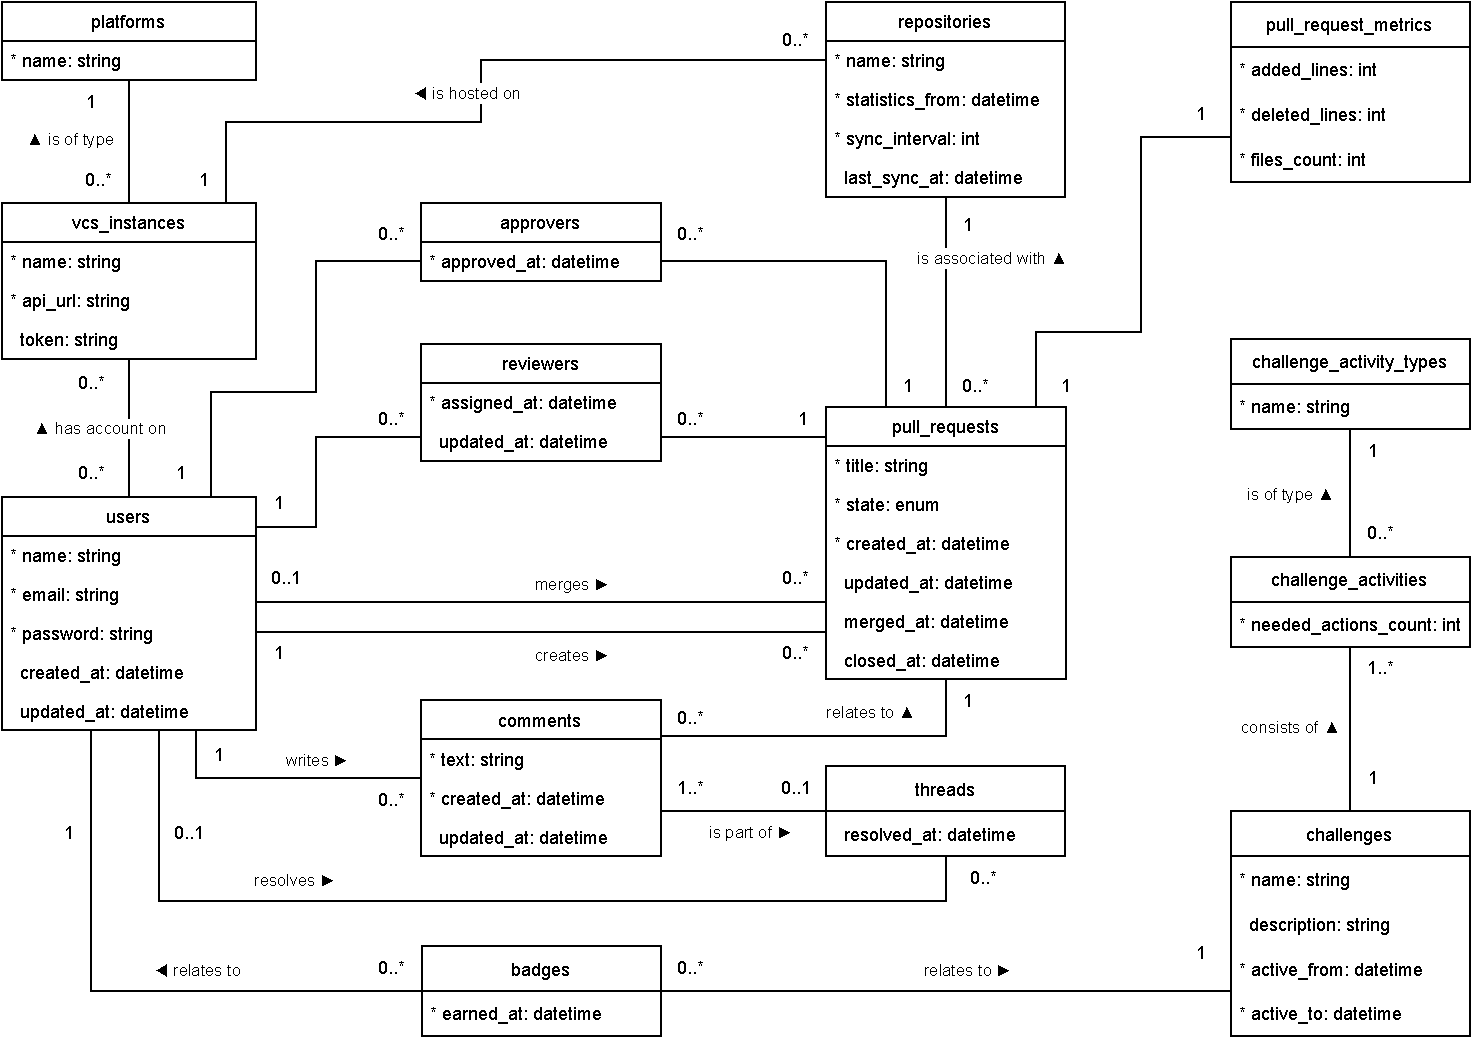
\includegraphics[height=\textheight]{images/domain-model.pdf}
    \end{figure}
\end{landscape}

\section{Technologie}

\subsection{PHP}

\subsection{Vue.js}

\subsection{Highcharts}


\chapter{Implementace}

\section{Použité nástroje}
Při implementaci bylo využito několik nástrojů, které zefektivňují práci při~vývoji softwaru. Pro hostování repozitáře se zdrojovým kódem byla využita platforma GitHub. Součástí repozitáře je rovněž automatizovaný bezpečnostní nástroj Dependabot, který byl aktivován za účelem průběžného monitorování závislostí projektu. Nástroj pravidelně kontroluje obsah souborů \texttt{composer.lock} a \texttt{package-lock.json} a v případě detekce známé bezpečnostní zranitelnosti v některé z použitých knihoven automaticky vytváří pull request s aktualizovanou verzí balíčku. Tím je zajištěna vysoká úroveň bezpečnosti aplikace bez nutnosti manuální kontroly všech externích komponent.

Jako vývojové prostředí byl při implementaci využit nástroj PhpStorm od~společnosti JetBrains. Tento editor je v komunitě PHP vývojářů široce využíván díky své robustní podpoře refaktoringu, pokročilé statické analýze kódu a integrovaným nástrojům pro ladění a testování. \cite{php-jetbrains} Pro zefektivnění vývoje nad frameworkem Laravel bylo prostředí rozšířeno o plugin Laravel Idea. Toto rozšíření poskytuje hlubší porozumění struktuře projektu, nabízí inteligentní doplňování kódu specifické pro Laravel a usnadňuje práci s Eloquent modely.

Pro zajištění konzistentního běhového prostředí byla využita technologie Docker. Aplikace je spolu se všemi svými závislostmi, jako je například webový server, zapouzdřena do izolovaných kontejnerů. Díky tomu bylo eliminováno riziko nekompatibility mezi lokálním prostředím a produkčním serverem. Definice infrastruktury v souboru \texttt{docker-compose.yml} navíc umožňuje rychlé sestavení aplikačních kontejnerů na jakémkoli zařízení s podporou Dockeru.


\section{Ukázky vybraných částí}

\section{Možná rozšíření}
Ačkoliv implementovaná aplikace splňuje veškeré požadavky definované v zadání diplomové práce, během procesu vývoje byly identifikovány oblasti, které by mohly být předmětem dalšího rozvoje. Pro zajištění efektivnější práce s rozsáhlejším množstvím dat se jako vhodné jeví rozšíření implementace o mechanismy řazení a filtrování v rámci tabulkových přehledů. Tímto způsobem by uživatelům bylo umožněno dynamicky organizovat zobrazené výstupy na základě specifických podmínek.

V rámci zvýšení uživatelské přívětivosti hlavního dashboardu by mohly být implementovány přímé odkazy do zdrojových systémů GitHub a GitLab. Jednotlivé záznamy v tabulkách by tak mohly obsahovat hypertextové odkazy směřující na detail konkrétního pull requestu v externím systému, čímž by byla zajištěna hlubší provázanost aplikace s verzovacími systémy. Kromě zmíněné integrace by dashboard mohl být vylepšen o perzistenci stavu filtrů (pro uživatele a časové období), které jsou v aktuálním řešení resetovány po~opuštění stránky. Implementací mechanismu pro ukládání jejich stavu by byla eliminována nutnost opakované konfigurace pohledů po každém přihlášení či přechodu mezi stránkami systému.

Vzhledem k tomu, že aplikace agreguje a normalizuje data z různých systémů pro správu verzí softwaru, disponuje značným množstvím informací s vysokou vypovídající hodnotou. Tato data mají vysoký potenciál pro další analytické využití, a proto je jako další možné rozšíření navrhováno napojení na~externí nástroje business intelligence. Data aplikace by následně mohla sloužit pro tvorbu komplexních reportů či hlubší analýzu trendů, kterou implementovaný systém v současné době nepokrývá.


\chapter{Testování}
V této kapitole budou nejprve představeny nástroje, které byly využity při~vývoji aplikace a které připívají k větší kvalitě vytvářeného kódu. Dále bude přiblížen průběh uživatelského testování, jeho výsledky a zpětná vazba od~účastníků.

\section{Automatické testy a kontroly}
Všechny níže uvedené testy a kontroly jsou integrovány do CI/CD procesu. Spouští se automaticky před sloučením změn a při přidání commitu do hlavní vývojové větve. Díky tomu je minimalizováno riziko zanesení chyb do produkčního prostředí a je garantováno dodržování stanovených standardů.

\subsection{Larastan}
Pro kontrolu PHP kódu byl zvolen nástroj Larastan. Jedná se o rozšíření populárního statického analyzátoru PHPStan, které je optimalizováno pro framework Laravel. Larastan při procesu analýzy kódu spouští aplikační kontejner, což mu umožňuje kromě statické analýzy datových typů a logické struktury programu kontrolovat i datové typy, které jsou běžně zjistitelné až za běhu aplikace. I díky tomuto přístupu je zajištěna podpora pro mnoho dynamických vlastností frameworku Laravel, což výrazně přispívá k typové bezpečnosti a robustnosti aplikace. \cite{Larastan}

\subsection{Laravel Pint}
Konzistence formátování PHP kódu je zajišťována nástrojem Laravel Pint. Jde o nástroj postavený na základech PHP CS Fixer, který však nabízí zjednodušenou konfiguraci a sady předpřipravených pravidel odpovídajících standardům pro vývoj PHP aplikací. Pint byl v rámci projektu konfigurován tak, aby kontroloval a opravoval styl zápisu kódu dle standardu PSR-12. Zajištění jednotného stylu, zahrnujícího pravidla pro odsazování, závorkování či deklaraci typů, je klíčové pro čitelnost kódu a efektivní spolupráci v týmu. \cite{Pint}

\subsection{ESLint, Prettier}
V kontextu klientské části aplikace slouží pro statickou analýzu kódu nástroj ESLint. Jeho účelem je identifikace problematických míst v komponentách frameworku Vue.js a v kódu jazyka JavaScript, která by mohla vést k chybám za běhu aplikace nebo k nekonzistencím v logice komponent.

Jako doplněk k nástroji ESLint je pro formátování zdrojového kódu frontendu využíván Prettier. Zatímco ESLint se zaměřuje na kvalitu a logickou správnost kódu, Prettier zajišťuje, aby všechny skripty a Vue.js komponenty měly jednotné formátování bez ohledu na to, kým byly napsány.

\subsection{PHPUnit}
Pro automatizované testování funkčnosti aplikace je využíván testovací framework PHPUnit. V současné fázi vývoje obsahuje projekt sadu základních testů, které byly součástí využitého Vue starter kitu. Tyto testy ověřují klíčové procesy, jako je registrace nového uživatele, změna přístupového hesla či~dostupnost hlavního dashboardu po úspěšném přihlášení. V budoucnu by však bylo vhodné tyto testy rozšířit na další funkcionality systému jako je například synchronizace dat se systémy pro správu verzí a ověření správnosti zobrazovaných metrik na dashboardu.

\section{Uživatelské testování}
V této sekci bude popsán proces a výsledky uživatelského testování vytvořené aplikace. Hlavním cílem této fáze bylo ověřit, zda je navržené uživatelské rozhraní dostatečně intuitivní pro koncové uživatele, a identifikovat potenciální nedostatky, které by mohly negativně ovlivnit uživatelskou přívětivost. Na základě získaných poznatků byly následně navrženy úpravy systému.

Před zahájením samotného testování byli účastníci seznámeni se skutečností, že předmětem hodnocení je samotný systém, nikoliv jejich individuální schopnosti či dovednosti. Testování ze zúčastnili celkem 4 uživatelé a bylo realizováno prezenční formou. To umožnilo sledovat bezprostřední reakce uživatelů a prováděné akce při plnění úkolů.

\subsection{Průběh testování}
Samotný proces testování byl rozdělen do několika fází:

\begin{enumerate}
    \item \textbf{Seznámení se systémem:} Každému účastníkovi byla nejprve představena podstata aplikace a její hlavní účel.
    \item \textbf{Průchod testovacími scénáři:} Uživatelům byly předány připravené scénáře obsahující sadu konkrétních úkolů, které měli v systému samostatně vykonat.
    \item \textbf{Závěrečný rozhovor:} Po dokončení všech úkolů byl s každým uživatelem veden strukturovaný rozhovor. Během této diskuse byly shromážděny subjektivní poznatky a náměty na funkční či vizuální vylepšení.
\end{enumerate}

\subsection{Testovací scénáře}

\subsubsection{Registrace do systému}
\begin{description}
    \item[\textcolor{black}{Modelová situace}] \hfill \\
        Dozvěděli jste se o nástroji, který umí porovnávat aktivitu vývojářů. Jste zvědaví, jak si stojíte oproti svým kolegům.
    \item[\textcolor{black}{Úkol}] \hfill
        \vspace{-2mm}
        \begin{enumerate}
            \item Zaregistrujte se do aplikace pod jménem Tomáš Novák, s e-mailem \mbox{tnovak@gmail.com} a libovolným heslem.
        \end{enumerate}
\end{description}

\subsubsection{Změna nastavení}
\begin{description}
    \item[\textcolor{black}{Modelová situace}] \hfill \\
        Při registraci jste omylem udělal ve své e-mailové adrese překlep a chtěl byste to napravit. Zároveň byste si chtěl změnit barevné schéma aplikace.
    \item[\textcolor{black}{Úkoly}] \hfill
        \vspace{-2mm}
        \begin{enumerate}
            \item Upravte svou e-mailovou adresu na t.novak@gmail.com
            \item Změňte vzhled aplikace na jiné barevné schéma.
        \end{enumerate}
\end{description}

\subsubsection{Zobrazení metrik}
\begin{description}
    \item[\textcolor{black}{Modelová situace}] \hfill \\
        Jste vedoucí vývojového týmu a chcete si zobrazit informace o aktivitách svého kolegy.
    \item[\textcolor{black}{Úkol}] \hfill
        \vspace{-2mm}
        \begin{enumerate}
            \item Zobrazte si metriky uživatele Lukáš Paukert od 20. ledna do 29. ledna.
        \end{enumerate}
\end{description}

\subsubsection{Správa sledovaných repozitářů}
\begin{description}
    \item[\textcolor{black}{Modelová situace}] \hfill \\
        Jste vedoucí vývojového týmu a chcete upravit seznam repozitářů, u kterých dochází ke sběru dat.
    \item[\textcolor{black}{Úkoly}] \hfill
        \vspace{-2mm}
        \begin{enumerate}
            \item Začněte od dnešního dne evidovat aktivity z repozitáře laravel/laravel z veřejné instance GitHub. Repozitář by se měl v systému zobrazovat pod jménem Laravel a data by měla být synchronizována každých 6~hodin.
            \item Odeberte repozitář Yii2 ze sledovaných projektů (včetně všech jeho dat).
        \end{enumerate}
\end{description}

\subsubsection{Přiřazení účtu ze systému pro správu verzí}
\begin{description}
    \item[\textcolor{black}{Modelová situace}] \hfill \\
        Jste vedoucí vývojového týmu a chcete novému uživateli přiřadit účet z verzovacího systému.
    \item[\textcolor{black}{Úkol}] \hfill
        \vspace{-2mm}
        \begin{enumerate}
            \item Přiřaďte uživateli Lukáš Paukert účet se jménem lukas.paukert z verzovacího systému GitLab provozovaným firmou DAMI.
        \end{enumerate}
\end{description}

\subsection{Průběh a vyhodnocení}

\chapter{Nasazení}
Tato kapitola se zabývá procesem zprovoznění a nasazení implementované aplikace. Nejprve bude podrobněji představen způsob využití technologie Docker. Následně bude uveden podrobný popis postupu pro spuštění systému v lokálním vývojovém prostředí a bude přiblíženo nastavení integrace s externími službami. V závěru kapitoly bude popsán proces nasazení aplikace s využitím cloudové platformy Render.

\section{Docker}
Celá aplikace je navržena pro provoz v izolovaném prostředí pomocí technologie Docker. Pro optimalizaci procesu sestavení je využíván mechanismus vícefázového sestavení. Tento přístup přináší následující klíčové benefity:

\begin{itemize}
    \item \textbf{Minimalizace času sestavení}: Díky rozdělení procesu do jednotlivých fází je umožněno využití již vytvořených vrstev. Tím je zamezeno opakování redundantních operací, což vede k výrazné časové úspoře při opětovném sestavování.
    \item \textbf{Snížení velikosti výsledného obrazu}: Do finálního obrazu se přenášejí pouze nezbytné soubory a zkompilovaný kód. Jelikož vývojové nástroje a meziprodukty zůstávají v předchozích fázích, je výsledná velikost obrazu minimalizována.
    \item \textbf{Oddělení prostředí}: Definice konkrétních cílů umožňuje z jediného konfiguračního souboru generovat specifické obrazy optimalizované pro odlišné účely.
\end{itemize}

\newpage
Pro účely této práce byly definovány dva cíle sestavení aplikace. Pro potřeby lokálního vývoje byl navržen cíl \texttt{development} a pro produkční prostředí byl specifikován cíl \texttt{production}.

\begin{itemize}
    \item \texttt{development}: Tato konfigurace je rozšířena o nástroj xDebug, který slouží k pokročilému ladění zdrojového kódu v jazyce PHP. Dále je integrováno prostředí Node.js verze 24 pro práci se závislostmi v jazyce JavaScript.
    \item \texttt{production}: Tento cíl byl nastaven jako výchozí a výsledný obraz je optimalizován s důrazem na minimalizaci jeho celkové velikosti. I z tohoto důvodu nebyly do obrazu zahrnuty vývojové nástroje, jako je například prostředí Node.js či adresář \texttt{node\_modules}.
\end{itemize}

Implementace cíle \texttt{production} je součástí výpisu kódu \ref{listing:dockerfile}. Proces sestavení začíná zkopírováním PHP závislostí a sestavených assetů z předchozích fází \texttt{vendor} a \texttt{node}. Následně jsou zkopírovány samotné zdrojové kódy aplikace a je provedeno nastavení vlastnických oprávnění. Příkazem \texttt{CMD} je definována sekvence kroků prováděných při startu kontejneru: nejprve jsou spuštěny databázové migrace, poté je vykonán příkaz \texttt{php artisan optimize} pro optimalizaci výkonu frameworku a nakonec je spuštěn webový server Apache.

\begin{listing}[h!]
    \caption{Cíl production z Dockerfile souboru}\label{listing:dockerfile}
    \begin{minted}{dockerfile}
FROM base AS production
WORKDIR /var/www/html

COPY --from=vendor /var/www/html/vendor/ ./vendor/
COPY --from=node /app/public/build/ ./public/build/
COPY . .

RUN chown -R www-data:www-data bootstrap/cache storage
RUN chmod -R 775 bootstrap/cache storage

CMD composer dump-autoload --optimize --no-dev --strict-ambiguous \
    && php artisan migrate --force \
    && php artisan optimize \
    && exec apache2-foreground
    \end{minted}
\end{listing}

\newpage
\section{Spuštění na lokálním prostředí}
Pro zprovoznění aplikace na lokálním prostředí je nutné provést kroky popsané v této sekci. Předpokladem pro úspěšné spuštění je nainstalovaný nástroj Docker a stažený repozitář se zdrojovým kódem projektu. Veškeré kroky by měly být prováděny v kořenovém adresáři projektu.

\begin{enumerate}
    \item vytvoření konfiguračního souboru \texttt{.env}, obsah lze zkopírovat ze vzorového souboru \texttt{.env.example}

    \item sestavení a spuštění aplikačních kontejnerů a databáze
    \begin{minted}{bash}
docker-compose up -d
    \end{minted}

    \item instalace závislostí pro backendovou část aplikace
    \begin{minted}{bash}
docker-compose exec php php composer install
    \end{minted}

    \item instalace závislostí pro JavaScript a sestavení single page aplikace
    \begin{minted}{bash}
docker-compose exec php npm install
docker-compose exec php npm run build
    \end{minted}

    \item vygenerování bezpečnostního klíče aplikace
    \begin{minted}{bash}
docker-compose exec php php artisan key:generate
    \end{minted}

    \item provedení databázových migrací pro vytvoření schématu
    \begin{minted}{bash}
docker-compose exec php php artisan migrate
    \end{minted}

    V rámci procesu migrace je v systému automaticky vytvořen administrátorský účet s následujícími přihlašovacími údaji:
    \vspace{-2mm}
    \begin{itemize}
        \item e-mail: \texttt{admin@devpulse.com}
        \item heslo: \texttt{password}
    \end{itemize}

    \item naplnění databáze testovacími daty (volitelné)
    \begin{minted}{bash}
docker-compose exec php php artisan db:seed 
    \end{minted}
\end{enumerate}

Po úspěšném provedení výše uvedených kroků je systém dostupný prostřednictvím webového prohlížeče na adrese \texttt{http://localhost/}. V případě potřeby lze všechny běžící kontejnery zastavit příkazem \texttt{docker-compose down}.

\section{Nastavení integrace s externími systémy}
Pro zajištění korektní synchronizace dat je nezbytné provést konfiguraci propojení s externími systémy pro správu verzí. Následující sekce popisují proces získání požadovaných autentizačních údajů a postup jejich nastavení v rámci vytvořené aplikace.

\subsection{GitHub App}
Integrace s platformou GitHub je realizována prostřednictvím registrace nové GitHub App, která může být vytvořena pod osobním účtem či v rámci organizace. V průběhu vytváření aplikace je vyžadováno vyplnění pouze jejího názvu a URL domovské stránky. Pro zajištění funkčnosti synchronizace je následně nezbytné udělit oprávnění v sekci \texttt{Repository permissions}, konkrétně pro~\texttt{Pull requests} v režimu \texttt{Read-only}.

Po dokončení registrace je aplikaci automaticky přidělen unikátní identifikátor \texttt{Client ID}. Pro získání privátního klíče je nutné provést jeho manuální vygenerování v administračním rozhraní aplikace. Tyto údaje je následně nezbytné vložit do~konfiguračního souboru \texttt{.env} pod klíči \texttt{GITHUB\_APP\_CLIENT\_ID} a \texttt{GITHUB\_APP\_PRIVATE\_KEY}. Závěrečným krokem je instalace aplikace do cílového účtu či organizace na platformě GitHub. Tímto úkonem je získán identifikátor \texttt{installation\_id}, který je nutné uvést při vytváření nové instance systému správy verzí v administraci vytvořené aplikace.

\subsection{GitLab}
V případě platformy GitLab je proces autentizace a následný přístup k datům realizován prostřednictvím přístupových tokenů. Z hlediska architektury vytvořeného systému je doporučeno využívat osobní či skupinové tokeny. V případě využití projektových tokenů by byla vyžadována konfigurace nové instance pro správu verzí pro každý sledovaný repozitář.

Při generování přístupového tokenu je nezbytné udělit oprávnění \texttt{read\_api}, které je vyžadováno pro synchronizaci dat. Na rozdíl od platformy GitHub není vygenerovaný token ukládán do konfiguračního souboru \texttt{.env}, ale je vkládán přímo do příslušného formuláře v průběhu vytváření nové instance systému pro správu verzí softwaru.

\subsection{E-mailový server}
Nedílnou součástí konfigurace produkčního prostředí je nastavení e-mailového serveru. Ve výchozím nastavení, které je definováno v souboru \texttt{.env.example}, je pro odesílání e-mailů nastaven ovladač \texttt{log}. Při využití tohoto ovladače avšak nedochází k reálné distribuci zpráv příjemcům, ale k jejich zápisu do~souboru \texttt{storage/logs/laravel.log}. Pro reálné odesílání e-mailů je nutné zvolit například ovladač \texttt{smtp}. V konfiguračním souboru \texttt{.env} musí být v tomto případě definovány hodnoty proměnných, které specifikují hostitele, port a autentizační údaje k příslušnému poštovnímu serveru. Seznam požadovaných proměnných je uveden na následujícím výpisu kódu.

\begin{minted}{bash}
MAIL_MAILER=smtp
MAIL_HOST=
MAIL_PORT=
MAIL_USERNAME=
MAIL_PASSWORD=
MAIL_FROM_ADDRESS=
\end{minted}

\section{Render}
Pro hostování aplikace byla zvolena platforma Render. Jedná se o cloudovou službu typu Platform as a Service, která umožňuje provozovat webové aplikace a související služby bez nutnosti správy vlastní serverové infrastruktury. V rámci realizovaného řešení je na této platformě hostována nejen samotná aplikační vrstva, ale také relační databáze MariaDB a plánovač úloh, který zajišťuje pravidelnou synchronizaci dat ze systémů pro správu verzí softwaru.

Celý proces nasazení byl plně automatizován díky přímé integraci s verzovacím systémem GitHub. Konfigurace zajišťuje, že při přidání commitu do~větve \texttt{master} dojde k automatickému sestavení a nasazení nové verze aplikace. Pro~korektní běh systému bylo nutné na straně poskytovatele definovat proměnné prostředí, které odpovídají obsahu lokálního souboru \texttt{.env}.

Z bezpečnostního hlediska je produkční verze, na rozdíl od lokálního vývojového prostředí, provozována výhradně na šifrovaném protokolu HTTPS. Výsledná aplikace byla zpřístupněna na doméně \texttt{devpulse.paukertlukas.cz}. Pro odesílání e-mailových notifikací byl systém propojen s externím SMTP serverem služby Mailtrap.

\chapter{Závěr}

\section{Vyhodnocení práce a splnění cílů}
Hlavním cílem této diplomové práce byl návrh a implementace open source webové aplikace určené k prezentaci aktivity vývojářů a ke zvýšení jejich motivace prostřednictvím gamifikačních prvků.

V teoretické části práce byly nejprve představeny systémy pro správu verzí softwaru GitHub a GitLab, přičemž pozornost byla věnována především jejich webovým API. Významnou část teoretické části dále tvořila rešerše metrik používaných pro měření kvality a produktivity práce vývojářů, v rámci níž byly představeny standardy SPACE a DORA. Na tuto rešerši navázala analýza možností motivace vývojářů a principů gamifikace. Následně byly specifikovány funkční a nefunkční požadavky kladené na vyvíjený systém a byla provedena analýza existujících řešení.

Na základě poznatků z teoretické části byla v praktické fázi navržena a následně implementována webová aplikace. Pro realizaci byly zvoleny moderní technologie zahrnující kontejnerizační nástroj Docker, programovací jazyk PHP s frameworkem Laravel a pro klientskou část Vue.js v kombinaci s knihovnou Inertia.js. Výsledný systém podporuje napojení na soukromé i veřejné instance platforem GitLab a GitHub, přičemž architektura aplikace byla navržena s důrazem na modularitu a možný budoucí rozvoj o další verzovací systémy. Kvalita zdrojového kódu byla průběžně validována nástroji pro statickou analýzu Larastan a ESLint. V závěru implementační fáze byly rovněž diskutovány směry dalšího možného rozšiřování aplikace.

Vytvořená aplikace byla podrobena uživatelskému testování, jehož výsledky sloužily jako podklad pro finální úpravy a optimalizace systému. Aplikace byla úspěšně nasazena do produkčního prostředí na platformě Render a její zdrojové kódy byly zveřejněny na platformě GitHub. Na základě výše uvedených skutečností lze konstatovat, že veškeré body definované v zadání diplomové práce byly splněny.

\section{Přínos a praktické využití}
Výsledkem práce je plně funkční aplikace připravená k nasazení do produkčního prostředí, která organizacím a vývojovým týmům poskytuje ucelený pohled na aktivity z procesu vývoje softwaru. Díky konsolidaci dat z různých zdrojů je systémem umožněna transparentní vizualizace aktivit napříč různými projekty a platformami. Při interpretaci jednotlivých metrik je však nezbytné zohlednit specifické procesy definované v rámci konkrétní organizace.

Přínosem je rovněž implementace gamifikačních mechanismů ve formě krátkodobých i dlouhodobých výzev a ocenění za aktivitu, které mohou přispět ke~zvýšení motivace uživatelů a podpořit zdravou soutěživost uvnitř týmů.

Realizací projektu bylo rovněž dosaženo prohloubení odborných znalostí autora v oblasti moderních webových technologií, konkrétně v rámci ekosystému Vue.js a Inertia.js a PHP frameworku Laravel.

\section{Budoucí rozvoj}
Ačkoliv implementované řešení splňuje veškeré požadavky definované v zadání práce, v průběhu vývoje a uživatelského testování byly identifikovány oblasti, které by mohly být předmětem dalšího rozvoje. Mezi navrhovaná rozšíření patří implementace mechanismů řazení a filtrování u tabulkových přehledů, perzistence filtrů či přímá integrace odkazů do zdrojových systémů. Vzhledem k charakteru agregovaných dat se rovněž nabízí napojení na nástroje business intelligence pro tvorbu komplexních reportů či hlubší analýzu trendů. Na základě zpětné vazby z testování by mohl být systém dále obohacen o grafické přehledy agregované po týdnech a měsících a o možnost manuální synchronizace. Ve vývoji aplikace je plánováno pokračovat a její funkcionalitu nadále rozšiřovat.


\appendix\appendixinit % do not remove these two commands

\chapter{Ukázky z vytvořené aplikace}

\begin{figure}[h]
    \centering
    \begin{minipage}[b]{0.48\linewidth}
        \caption{Proces registrace I.}
        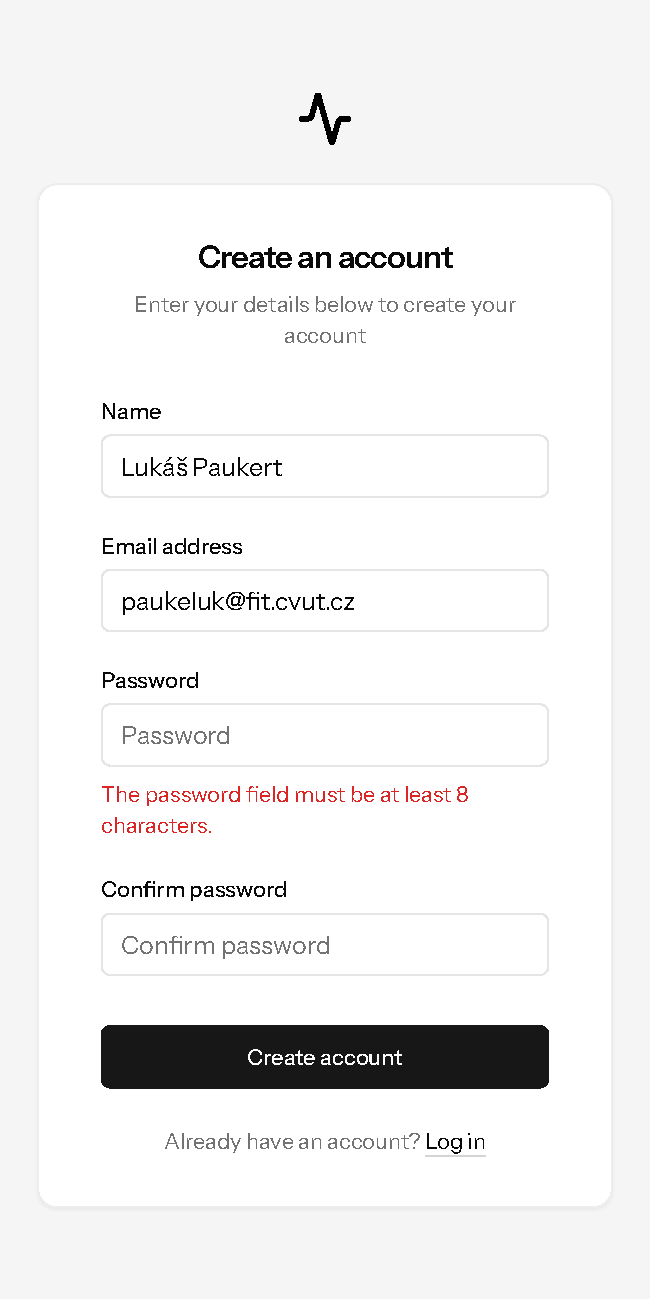
\includegraphics[width=0.99\linewidth]{images/appendix/registration.pdf}
    \end{minipage}
    \hfill
    \begin{minipage}[b]{0.48\linewidth}
        \caption{Proces registrace II.}
        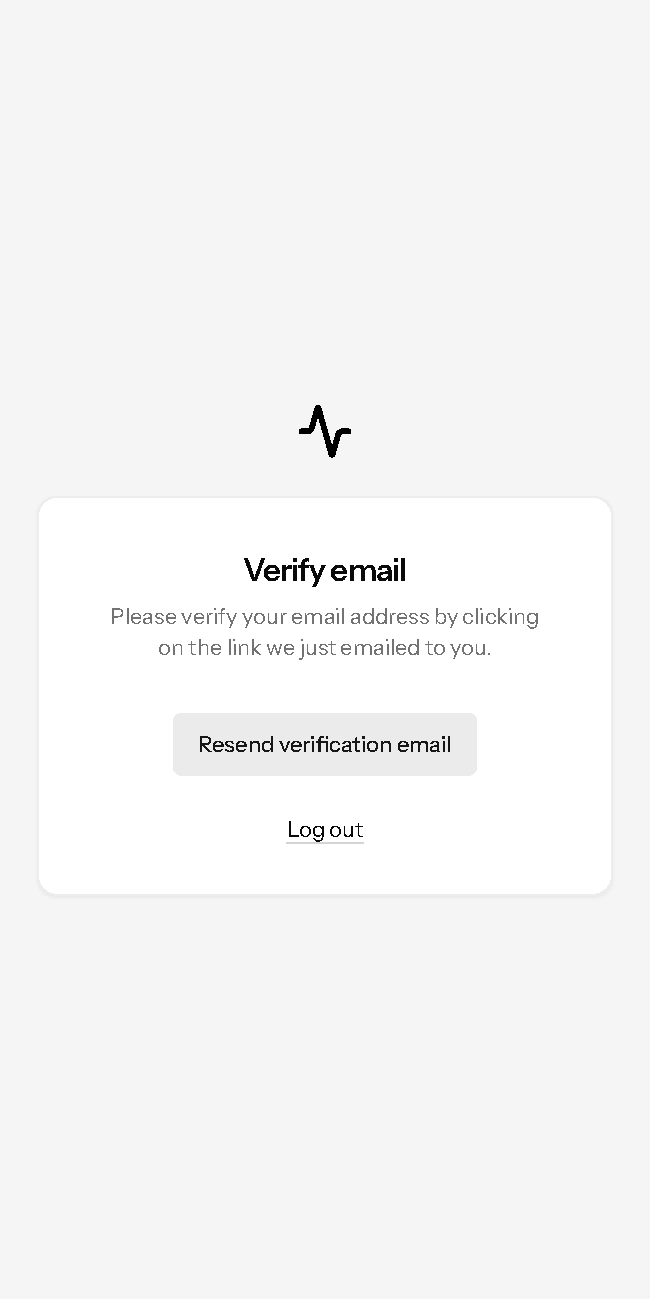
\includegraphics[width=0.99\linewidth]{images/appendix/verification.pdf}
    \end{minipage}
\end{figure}

\begin{figure}[h]
    \caption{Hlavní stránka aplikace}
    \centering
    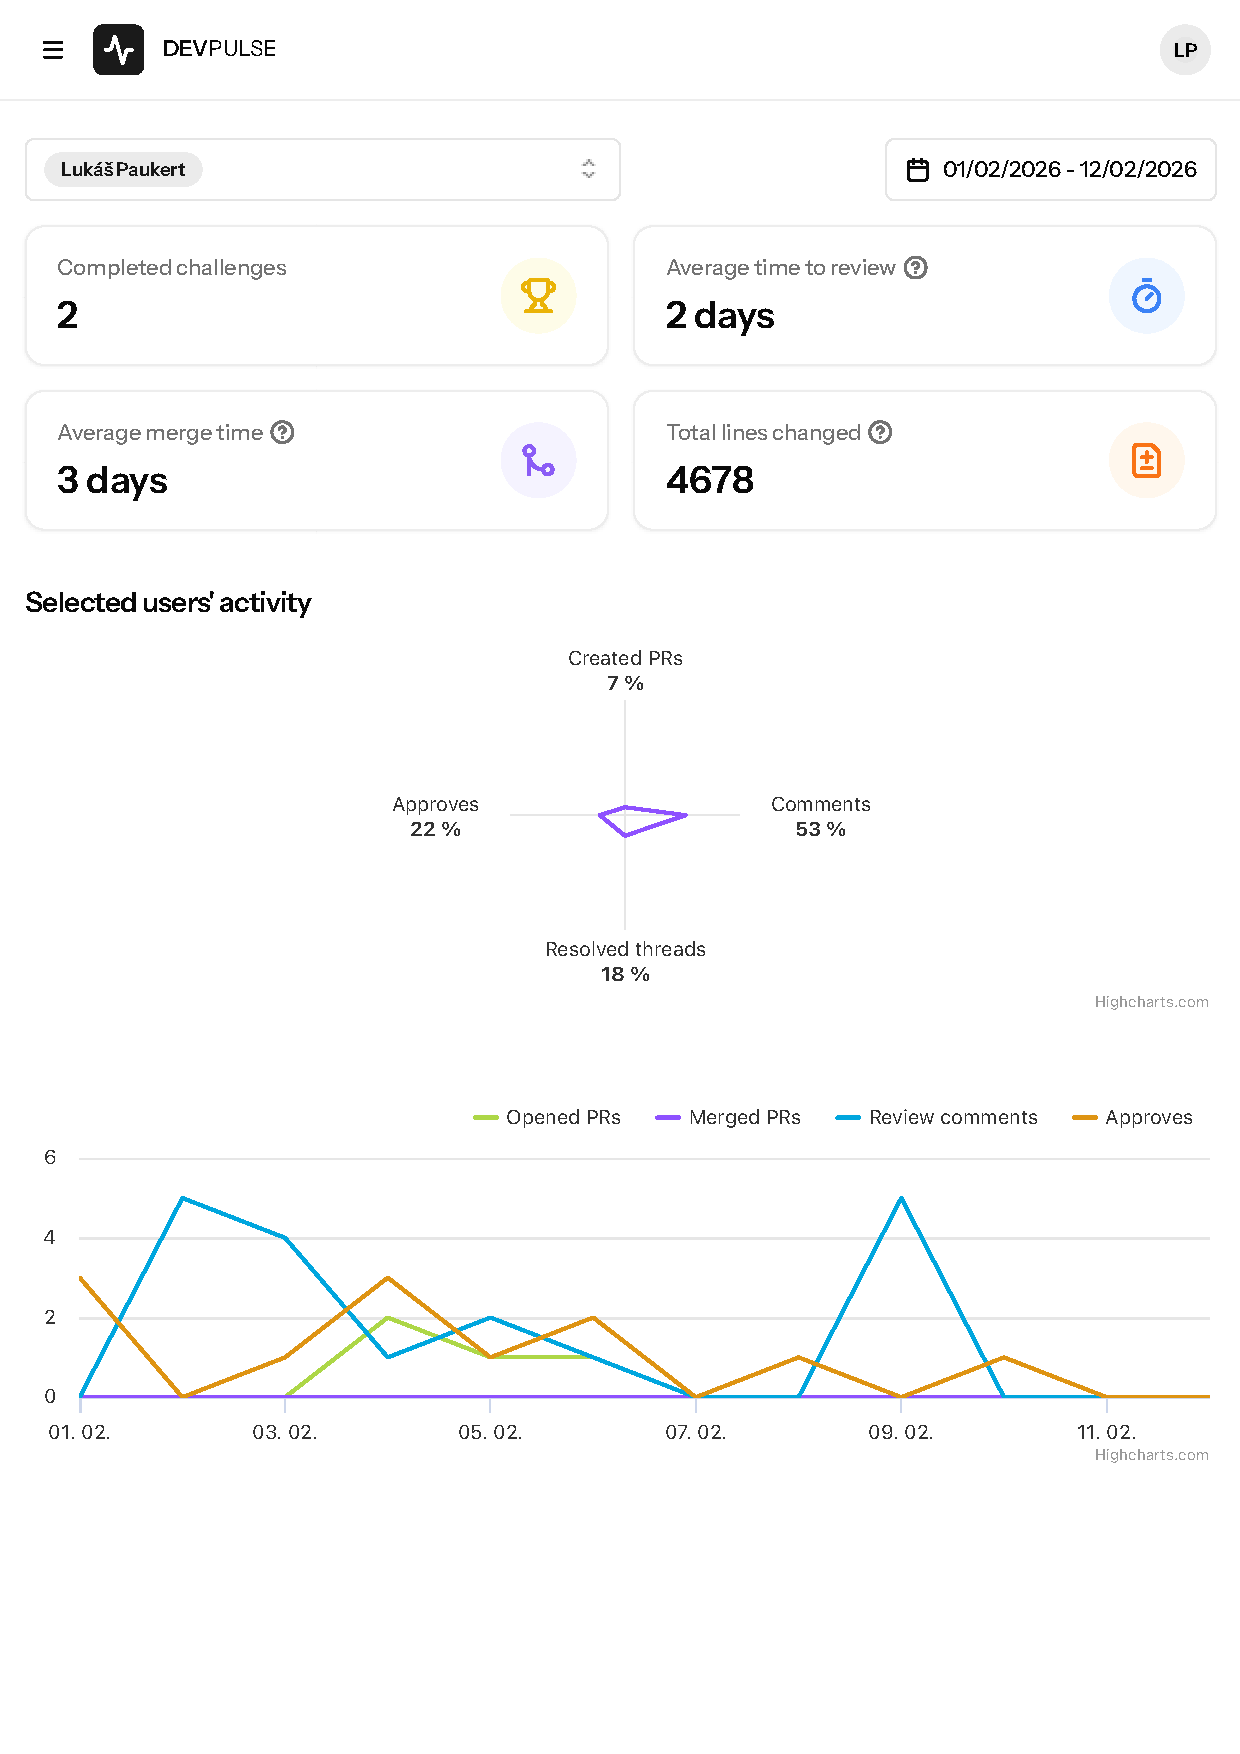
\includegraphics[width=0.995\linewidth, trim={0 110pt 0 0}, cfbox=gray 0.5pt 0pt]{images/appendix/dashboard.pdf}
\end{figure}

\begin{figure}[h]
    \caption{Přiřazování VCS účtů uživatelům}
    \centering
    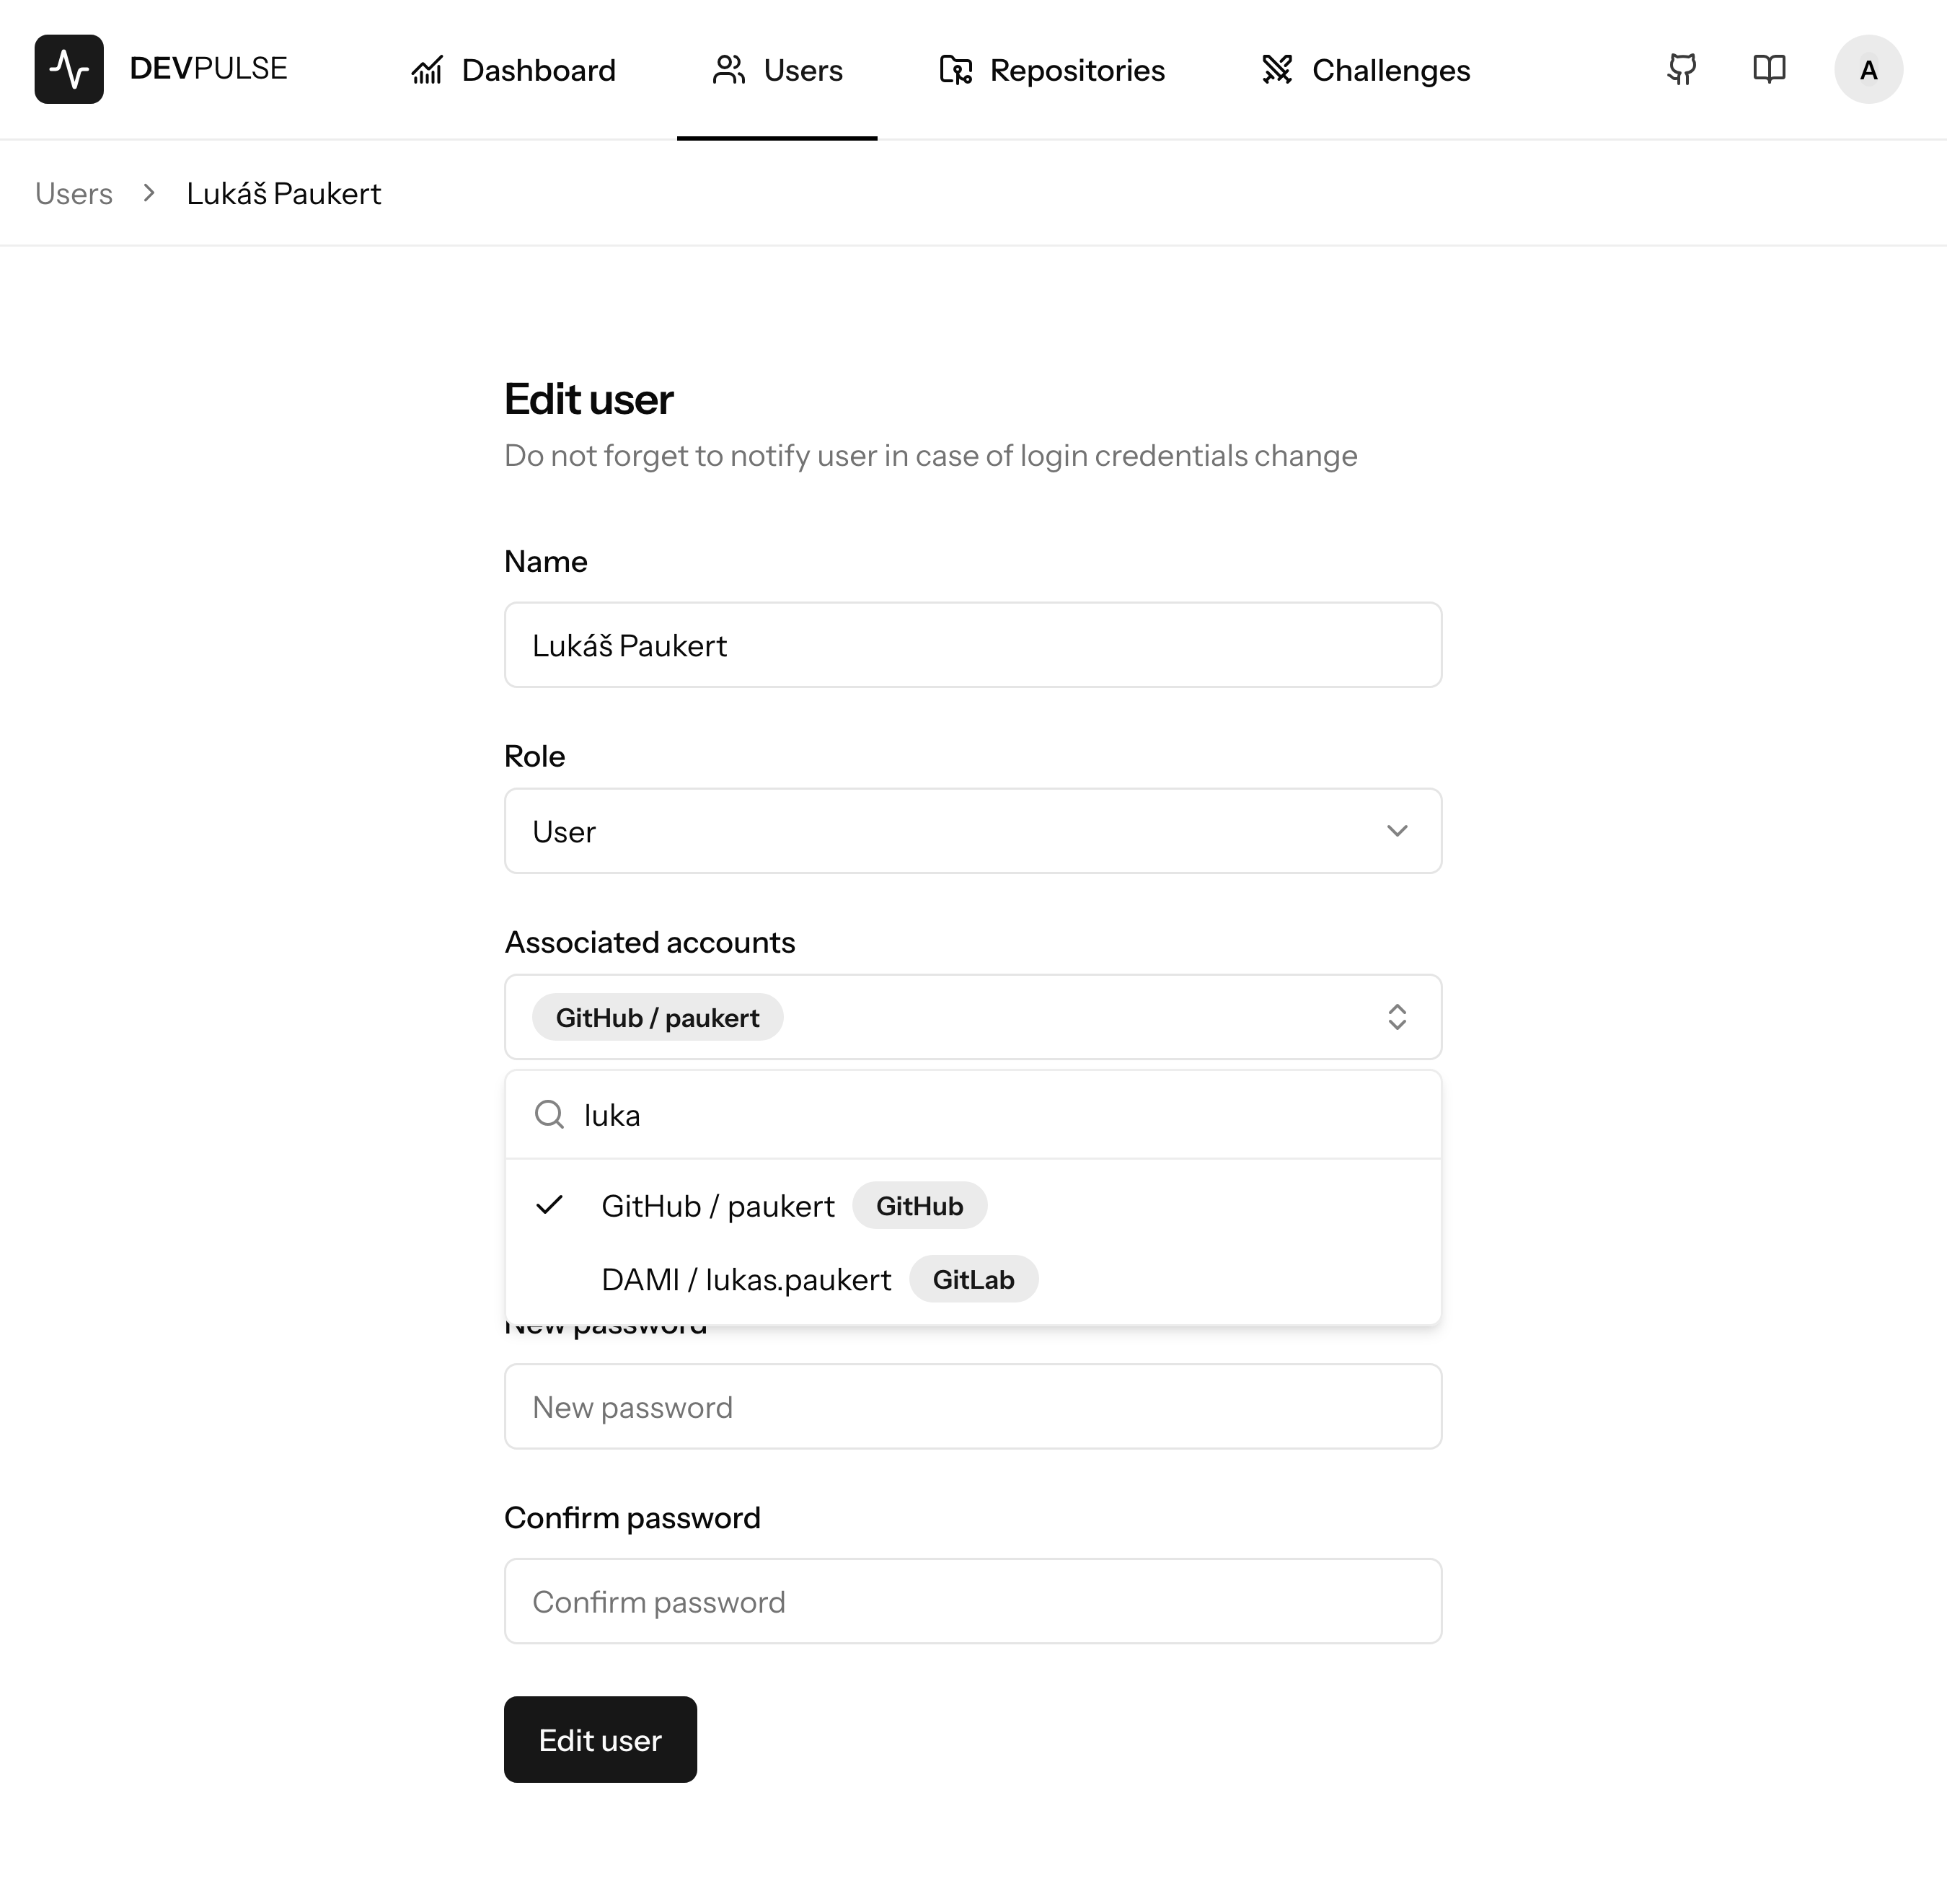
\includegraphics[width=0.995\linewidth, cfbox=gray 0.5pt 0pt]{images/appendix/account-assignment.png}
\end{figure}

\begin{figure}[h]
    \centering
    \begin{minipage}[b]{0.48\linewidth}
        \caption{Nastavení I.}
        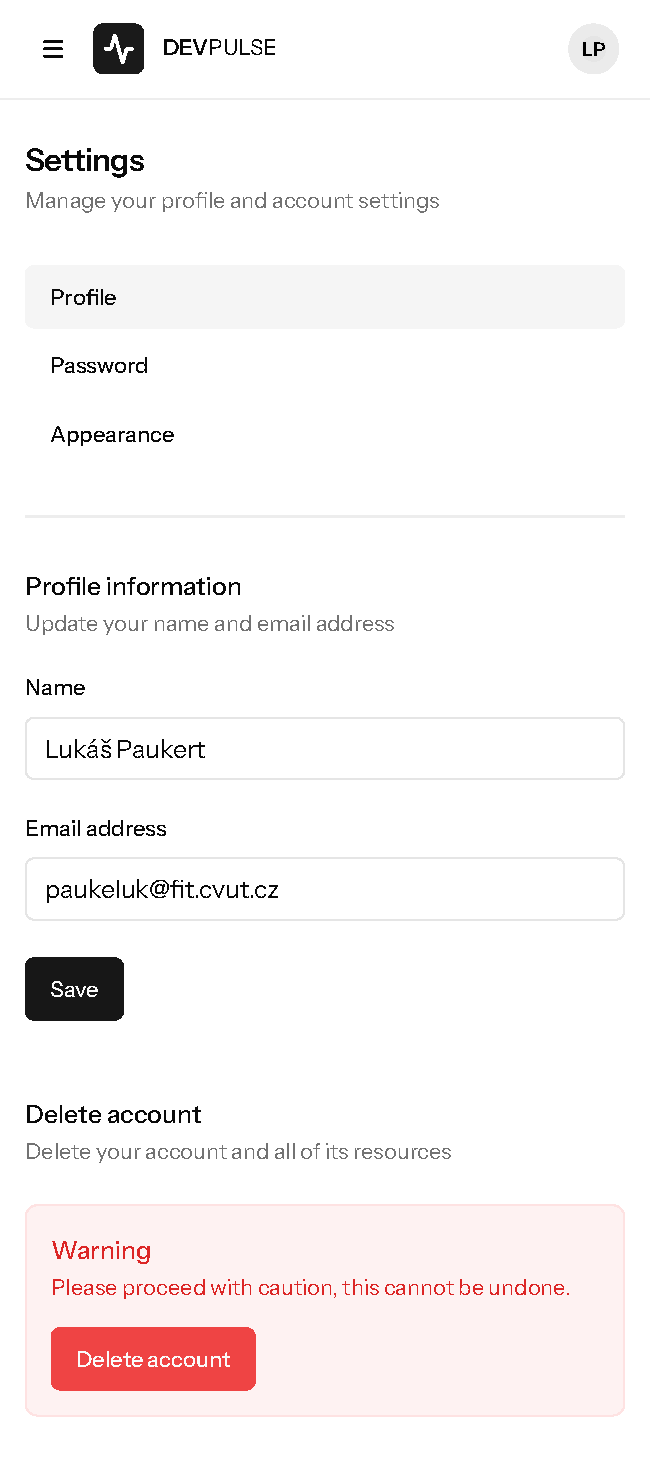
\includegraphics[width=0.99\linewidth, cfbox=gray 0.5pt 0pt]{images/appendix/profile.pdf}
    \end{minipage}
    \hfill
    \begin{minipage}[b]{0.48\linewidth}
        \caption{Nastavení II.}
        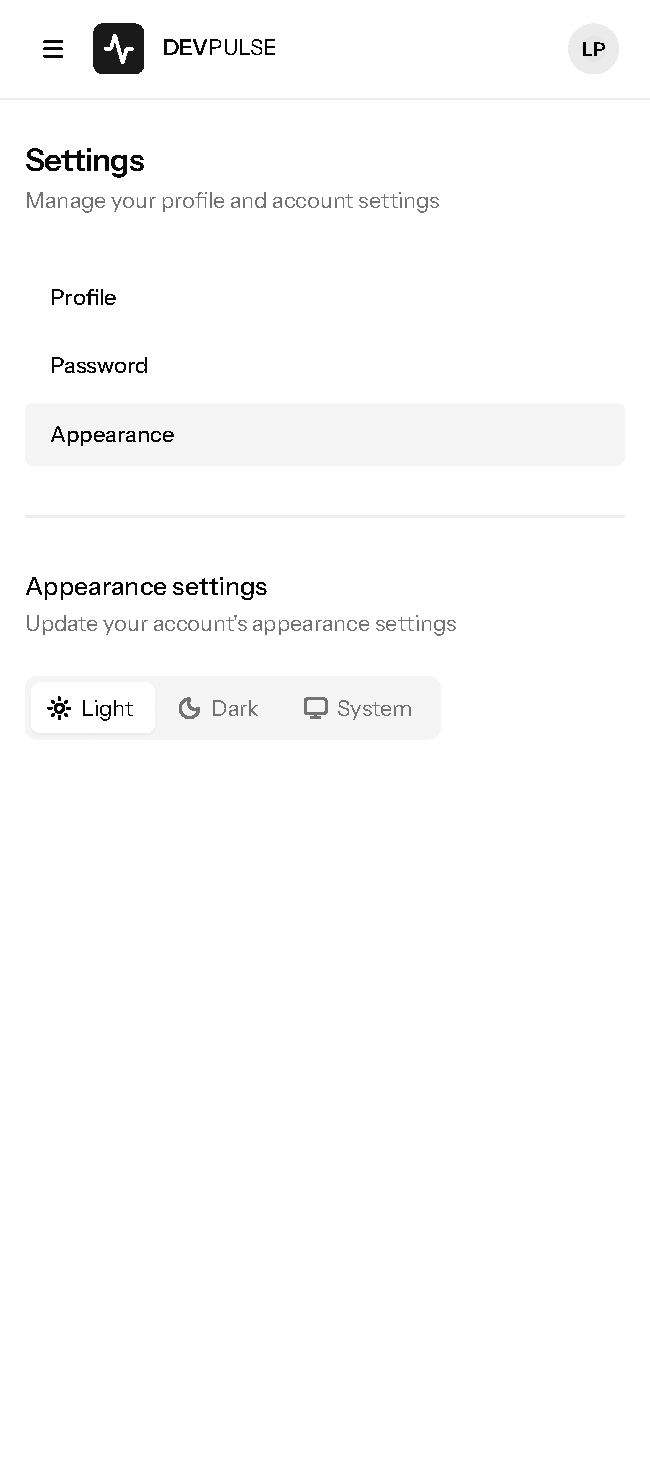
\includegraphics[width=0.99\linewidth, cfbox=gray 0.5pt 0pt]{images/appendix/appearance.pdf}
    \end{minipage}
\end{figure}
 % include `appendix.tex' from `other/' subdirectory

\backmatter % do not remove this command

\printbibliography % print out the BibLaTeX-generated bibliography list

\chapter{Obsah příloh}
% Contents of the attachment

	\dirtree{%
		.1 /.
		.2 readme.txt\DTcomment{stručný popis obsahu média}.
		.2 src.
		.3 app\DTcomment{zdrojové kódy implementace}.
		.3 thesis\DTcomment{zdrojová forma práce ve formátu \LaTeX{}}.
		.2 text\DTcomment{text práce}.
		.3 thesis.pdf\DTcomment{text práce ve formátu PDF}.
	}
 % include `medium.tex' from `other/' subdirectory

\end{document}
